\documentclass[a4paper,11pt]{article}
\usepackage[italian]{babel}
\usepackage[utf8]{inputenc}
\usepackage[margin = 1.4in]{geometry}
\usepackage{amsmath}
\usepackage{centernot}
\usepackage{amsfonts}
\usepackage{tcolorbox}
\usepackage{float}
\usepackage[font=scriptsize]{caption}
\usepackage[framemethod=tikz]{mdframed}
\newmdenv[innerlinewidth=0.5pt,roundcorner=4pt,linecolor=lightgray,innerleftmargin=6pt,
innerrightmargin=6pt,innertopmargin=6pt,innerbottommargin=6pt]{myblock}
\begin{document}
\title{\textbf{Curve calibrazione diodi}

2°turno tavolo 5}
\author{Stefano Doria 0001093903 \and Giuseppe Luciano 0001077643}

\date{Novembre 2024}

\maketitle

\section{Abstract}
Nella seguente prova si è tentato di ricostruire le caratteristiche I-V di due diodi a semiconduttore (Si, Ge) in polarizzazione diretta. In aggiunta si è tentato di ricavare la corrente di saturazione inversa ed il prodotto fra il fattore di idealità e la tensione termica per le due componenti ottenendo [valori] con un accordo di [valori]. Inoltre è stata preventivamente compiuta anche una calibrazione degli strumenti di misurazione utilizzati per assicurarsi che non vi fosse uno sfasamento fittizio durante la fase di misurazione di una stessa grandezza. Dopo a ottenendo una pendenza di (1.00 $\pm$ 0.02) ed intercetta di ($\pm$)  con un accordo di [valori].

\section*{Introduzione}
In questo esperimento è stata analizzata la caratteristica I-V di due diodi a semiconduttore, al silicio (Si) e germanio (Ge), variando l’intensità di corrente continua tramite un potenziometro. 

Un diodo a giunzione p-n consiste in due regioni contigue con drogaggi specifici, ottenuti introducendo impurezze in concentrazioni tipiche di $10^{14} - 10^{16} \, \mathrm{\frac{atomi}{cm^3}}$. La regione di tipo $n$ è solitamente drogata con atomi pentavalenti (come fosforo o arsenico), che forniscono elettroni aggiuntivi e aumentano la concentrazione di portatori di carica negativa. La regione di tipo $p$, invece, è drogata con atomi trivalenti (come boro o gallio), che creano lacune, ovvero assenza di elettroni di legame nel reticolo cristallino del silicio, e agiscono come portatori di carica positiva.

Queste regioni quando affiancate generano una giunzione con un potenziale di contatto. Quando si applica una tensione esterna in polarizzazione diretta, ossia si collega la regione p con il terminale
positivo e la regione n con quello negativo, si viene a ridurre ulteriormente la barriera di potenziale che le cariche devono superare per oltrepassare la regione di separazione. In questo modo le cariche libere (elettroni e lacune attratte dal potenziale agli estremi del dispositivo) possono attraversare la giunzione con minori difficoltà facendo passare corrente, come descritto in [1].

La caratteristica I-V di un diodo polarizzato direttamente segue un andamento esponenziale, descritto nel modello ideale dalla relazione\eqref{eq::diodo_ideale}:
\begin{equation}
\label{eq::diodo_ideale}
I=I_O(e^{\frac{V_D}{\eta V_T}}-1) \approx  I_O e^{\frac{V_D}{\eta V_T}}
\end{equation}

dove $I_0$ è la corrente di saturazione inversa, $V$ la tensione applicata, $V_T = \frac{kT}{q}$ la tensione termica, e $\eta$ il parametro di idealità del diodo, come discusso in [1].

Nella pratica, tuttavia, effetti di non idealità, come la resistenza del materiale semiconduttore e le perdite interne, alterano l'andamento della corrente, specialmente ai valori più alti, rispetto a quanto previsto dal modello  producendo correnti inferiori.
	
\section{Medoto Sperimentale}
Durante lo svolgimento della prova si è utilizzato un generatore di tensione continua che erogava una differenza di potenziale fissa di 5V quindi per modulare la corrente all'interno del circuito, realizzato su una breadboard, è stato impiegato un potenziometro da 1 $\mathrm{ K\Omega}$ impiegando come strumenti di misura un multimetro ed un oscilloscopio oscilloscopio. Per avere un'idea migliore dell'apparato sperimentale si faccia riferimento alla figura \ref{fig::apparato}. 

Si è inoltre provato ad effettuare delle misurazioni con generatore di tensione spento per valutare la presenza di un eventuale fondo legato ad una possibile corrente introdotta dall'amperometro.

\begin{figure}[ht]
    \centering
    \begin{minipage}{0.45\textwidth}
        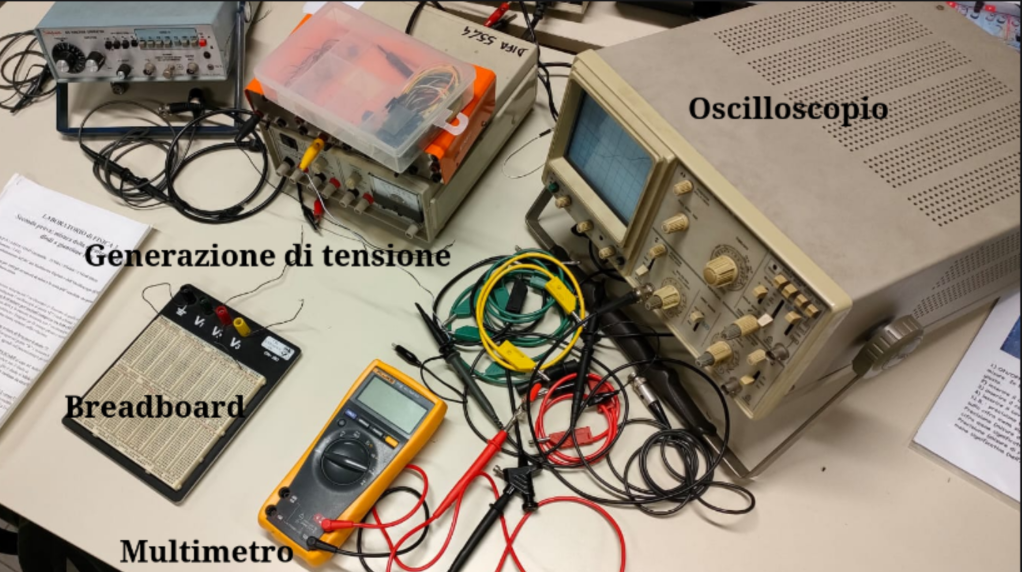
\includegraphics[width=\textwidth]{pictures/apparato.png}
    \end{minipage}%
    \hfill
    \begin{minipage}{0.45\textwidth}
        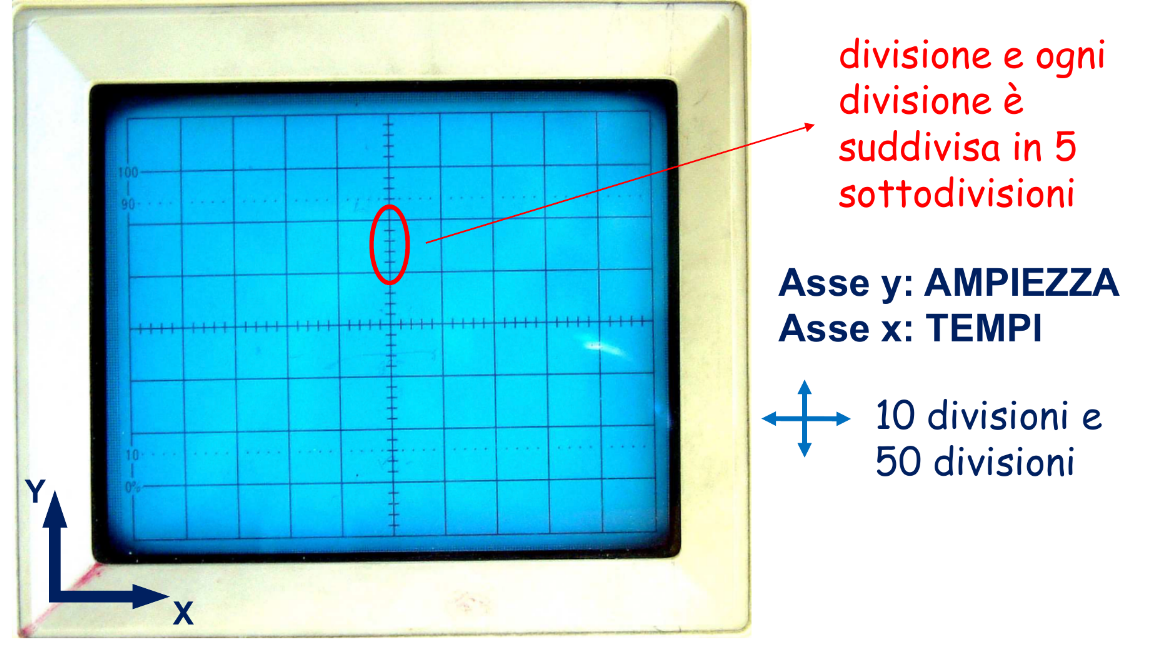
\includegraphics[width=\textwidth]{pictures/oscilloscopio.png}
    \end{minipage}
    \caption{\textit{\textcolor{gray}{A sinistra, l'immagine mostra l'apparato sperimentale impiegato, con l'oscilloscopio in alto a destra, il multimetro a sinistra, la breadboard in basso e il generatore di tensione al centro. A destra, si vede il display dell'oscilloscopio, evidenziando le divisioni e le suddivisioni.}}}
    \label{fig::apparato}
\end{figure}


    Dopo aver realizzato il circuito sulla breadboard in una configurazione analoga a quella mostrata in figura \ref{fig::circuito} ma con la differenza che si sono cortocircuitati i punti A e B e si è collegato l'oscilloscopio nel punto C, si è proceduto costruendo la curva di calibrazione misurando con il multimetro e con l'oscilloscopio lo stesso valore di tensione al variare della resistenza di carico del potenziometro. Per facilitare l'operazione si è cercato di  selezionare i valori di più facile lettura sull'oscilloscopio, ossia quelli che si presentavano in corrispondenza delle linee presenti sul display, si guardi la figura \ref{fig::apparato}, accertandosi che il segnale fosse sempre stabile e pulito.
\begin{figure}
	\centering
	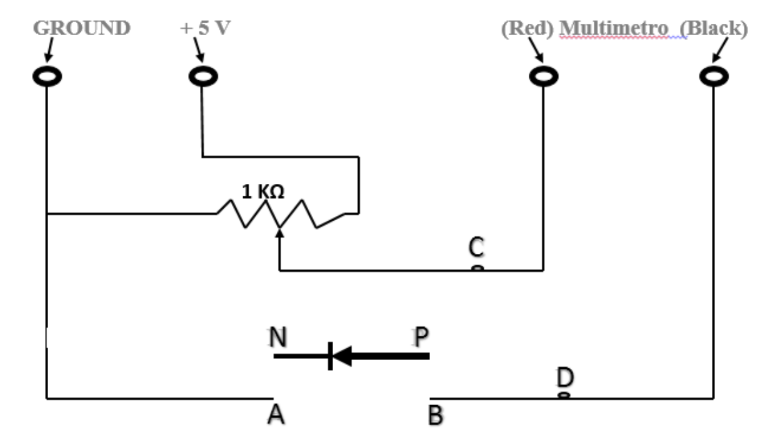
\includegraphics[width=0.6\textwidth]{pictures/circuito.png}	\caption{\textit{\textcolor{gray}{La foto mostra lo schema del circuito nella configurazione di diodo inserito nei punti indicati con le lettere A e B. Invece il circuito per la calibrazione è stato ottenuto collegando
    l'oscilloscopio al punto C e cortocircuitando i punto A-B.}}}
    \label{fig::circuito}
\end{figure}
Si è quindi proceduto valutando la curva di calibrazione dei diodi. Per farlo è stato modificato il circuito precedentemente creato realizzando la configurazione visibile in figura \ref{fig::circuito} impostando il multimetro per lavorare in configurazione di corrente continua. Per evitare di danneggiare tali dispositivi si è prima verificato che il potenziometro fosse settato in modo da avere una resistenza di carico di 5 $\mathrm{k\Omega}$ sufficiente a garantire che la corrente nel circuito non fosse troppo elevata. Si è poi proceduto come in precedenza campionando la d.d.p e la corrente ai capi del dispositivo, al variare della resistenza di carico, selezionando i valori che risultavano più facilmente leggibili, ripetendo la stessa procedura anche per l'altro diodo. Per facilitare la presa dati è stato inoltre necessario variare progressivamente il valore assunto da ogni divisione in base alla misura che si stava effettuando. Nel farlo si è prestato attenzione ad evitare i segnali che si trovassero nella prima o nell'ultima divisione, si faccia riferimento alla figura \ref{fig::apparato}, a causa della distorsione maggiore del segnale per via delle caratteristiche costruttive dell'oscilloscopio.

Si è inoltre prestato attenzione ad immettere nel circuito una tensione compresa fra 0.05 V e 0.8 V per non danneggiare i diodi cercando di concentrare quante più misure possibili in prossimità di piccoli valori di corrente e di potenziale per non avvicinarsi alla regione dove il comportamento ideale risulta essere peggio descritto. Per tale motivazione ad ogni nuovo punto si è verificato come cambiasse la curva, cercando di individuare la regione dopo la quale la descrizione del fenomeno peggiorava. Nonostante questo sono stati comunque campionati valori a tensioni più alte per verificare che il comportamento qualitativo seguisse quanto atteso, ossia di diminuzione della corrente rispetto a quanto previsto dalla legge del diodo ideale.


\section{Risultati}

\subsection{Dati}

Si riportano nella tabella \ref{tab::dati} i dati acquisiti tramite oscilloscopio e multimetro per la calibrazione di questi e per la misura della caratteristica dei due diodi. Gli errori sono stati associati come da specifiche di multimetro e oscilloscopio, trattandoli rispettivamente come strumentali e casuali. 

 Durante la prova è stato inoltre utilizzato un oscilloscopio, il GOS-622B (modello 1), per stimare la d.d.p ai capi del diodo, il cui zero è stato fissato a $5 \mathrm{mV}$. Vi erano diverse possibili scelte per il valore di ogni divisione presente sul display (5V, 2V, 1V, 0.5V, 0.2V, 0.1V, 50mV, 20mV, 10mV, 5mV). Nel calcolo dell'incertezza per l'oscilloscopio l'errore stimato sulla lettura è stato preso come un decimo del fondo scala, in quanto il segnale si presentava in modo molto stabile e con rumore minimo(una buona risoluzione visiva sullo schermo dello strumento). 
 
 È stato impiegato anche un multimetro, il FLUKE 77 IV, con una risoluzione di $0.1\mathrm{mV}$ sulle misure di potenziale in corrente continua su fondoscala di $600\mathrm{mV}$ e $1\mathrm{mV}$ su fondoscala di $6\mathrm{V}$ con accuratezza dello 0.3 $\%$ sulla lettura a cui si dove sommare la risoluzione, mentre per le misure con l'amperometro in corrente continua la risoluzione è di $0.01\mathrm{mA}$ su fondoscala di $60\mathrm{mA}$ ed accuratezza del 1.5 $\%$ sulla lettura a cui sommare il doppio della risoluzione. Inoltre si è usata un'incertezza sullo zero di 0.0005 mV, avendo usato un fondo scala di 0.005 mV per misurarlo. 

\begin{table}[h!]
    \centering
 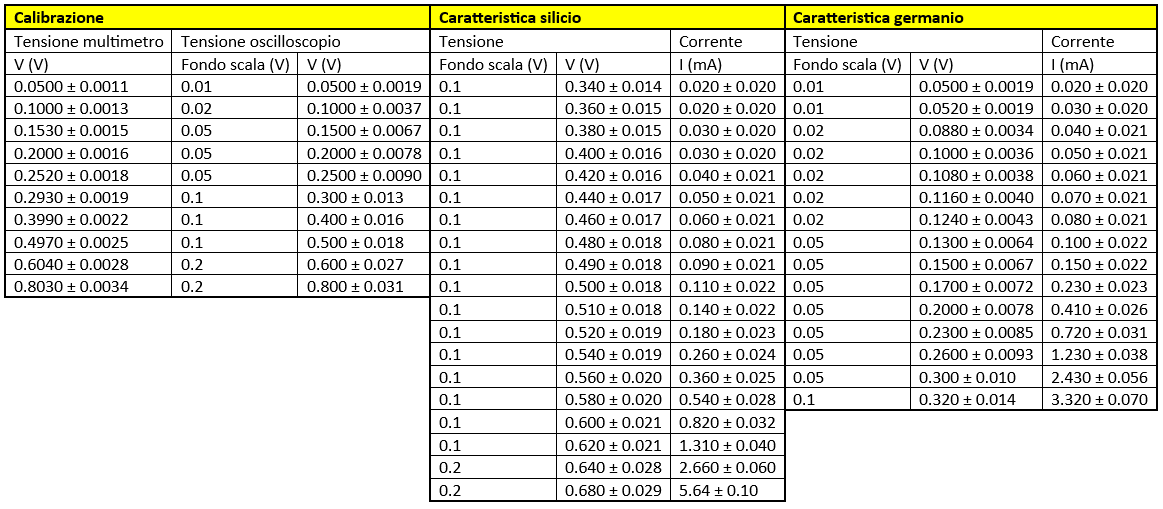
\includegraphics[width=1. \textwidth]{pictures/tabella.png}
    
    \caption{\textit{\textcolor{gray}{A partire da sinistra si riportano i dati per la calibrazione, quelli per la caratteristica del silicio ed infine quelli per il germanio. Si fa notare che gli errori da oscilloscopio sono casuali, mentre quelli da multimetro sono massimi.}}}
        \label{tab::dati}
\end{table}


\subsection{Analisi Dati} 

Nella figura \ref{graph::calibrazione} si riporta il grafico con il fit lineare sui dati di tensione acquisiti per calibrare multimetro e oscilloscopio. 

\begin{table}[h!]
	\centering
  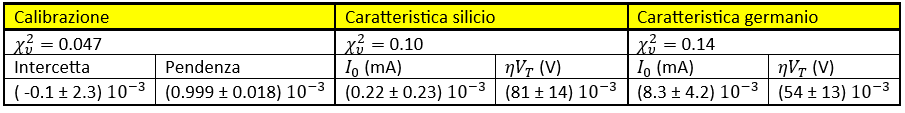
\includegraphics[width=1.\textwidth]{pictures/risultati2.png}	\caption{\textit{\textcolor{gray}{La tabella mostra i risultati ottenuti dai fit riportando da sinistra i risulati dalla calibrazione, la caratteristica del silicio e quella del germanio}}}
    \label{tab::risultati}
\end{table}

Le figure \ref{graph::silicio} e \ref{graph::germanio} riportano i grafici con i dati di tensione e corrente per i due diodi e le relative curve di caratteristica ottenute tramite fit della curva descritta dall'equazione \ref{eq::diodo_ideale}. In entrambi i casi i fit sono stati effettuate su un insieme ristretto di punti rispetto al totale dei dati acquisti, a causa degli effetti non ideali presenti oltre la tensione di soglia di un diodo.

Si specifica inoltre come nella misura della corrente a generatore spento si sia ottenuto un valore non nullo, probabilmente a causa delle caratteristiche del multimetro, di $I_sp=(0.02 \pm 0.02)$ $ \mathrm{mA}$ che risulta comunque compatibile con corrente nulla. 
% Figura della calibrazione
\begin{figure}[H]
    \centering
    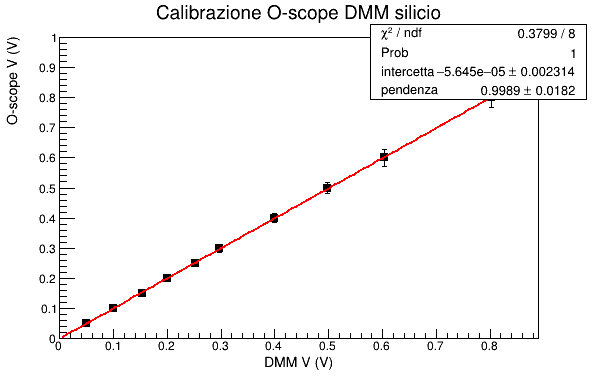
\includegraphics[width=0.5\textwidth]{pictures/calibrazione.png}
    \caption{\textit{\textcolor{gray}{Il grafico mostra le misure di tensione ottenute dal multimetro (in ascissa) e dall'oscilloscopio (in ordinata), con la relativa calibrazione.}}}
    \label{graph::calibrazione}
\end{figure}

% Grafici delle caratteristiche dei diodi
\begin{figure}[H]
    \centering
    \begin{minipage}{0.48\textwidth}
        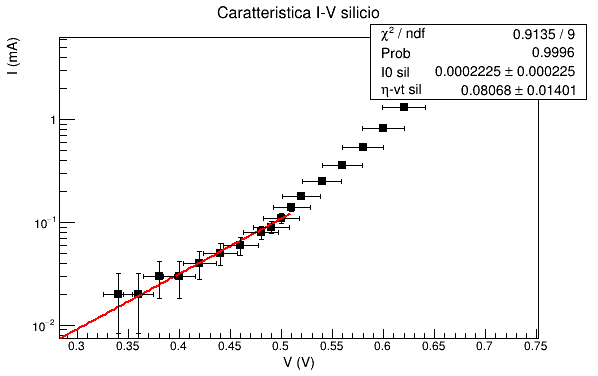
\includegraphics[width=\textwidth]{pictures/silicio.png}
        \caption{\textit{\textcolor{gray}{ }}}
        \label{graph::silicio}
    \end{minipage}
    \hfill
    \begin{minipage}{0.48\textwidth}
        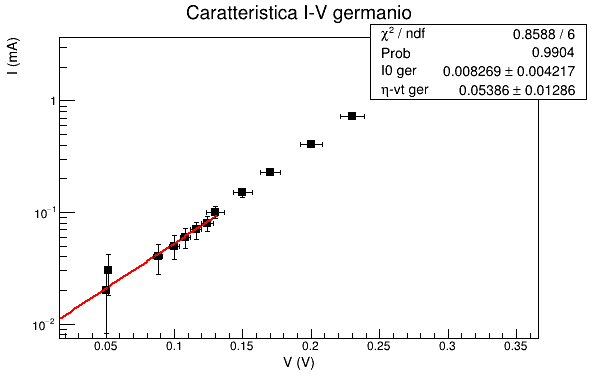
\includegraphics[width=\textwidth]{pictures/germanio.png}
        \caption{\textit{\textcolor{gray}{ }}}
        \label{graph::germanio}
    \end{minipage}
    \caption{\textit{\textcolor{gray}{I grafici mostrano le curve caratteristica dei diodi con asse delle ordinate logaritmico ed il relativo fit esponeziale rispettivamente per il diodo al silicio a sinistra e germanio a destra.}}}
\end{figure}



\section{Conclusioni}

Si è verificato che la calibrazione tra multimetro e oscilloscopio seguisse una retta di intercetta ($\pm$) e pendenza ($\pm$), con un $\tilde\chi^2$ di . Valori che corrispondono a quelli attesi.

Per la caratteristica del diodo al silicio i valori restituiti dal fit sono: $I_0$ ($\pm$), $\eta V_t$ ($\pm$) e fondo ($\pm$), con $\tilde\chi^2$. 

 SI sottolinea poi come nel caso del gemanio si osserva in modo più evidente come per alti valori di tensioni la pendenza della retta che congiunge i vari punti appare minore, effetto comunque presente anche nel caso dell'altro diodo.

 %RIVEDERE PARTE SU ANDAMENTI CARATTERISTICHE DIODI

Si osservano tendenzialmente dei valori di $\tilde\chi^2$ molto inferiori all'unità, aspetto che suggerisce una abbondante sovrastima delle incertezze. Tale sovrastima sarebbe da attribuire al fatto che i valori diverse misure risultano confrontabili con la risoluzione degli strumenti usati. 

\section{Bibliografia}

\end{document}